\documentclass[12pt]{article}
\usepackage[a4paper,top=3cm,left=2cm,right=2cm,bottom=2cm]{geometry}
\usepackage[utf8]{inputenc}
\usepackage[czech]{babel}
\usepackage[unicode]{hyperref}
\usepackage{graphicx}
\usepackage{float}
\usepackage{subcaption}
\begin{document}

	\begin{titlepage}
		\begin{center}
			
\includegraphics[height = 96pt]{img/FIT_barevne_CMYK_CZ.pdf} \\

			\begin{LARGE}
				\textbf{Vysoké učení technické v~Brně} \\
			\end{LARGE}

			\begin{Large}
				\textbf{Fakulta informačních technologií} \\
			\end{Large}

			\begin{large}
				Mikroprocesorové a vestavěné systémy \\
				2020~/~2021
			\end{large}

			\vspace{\stretch{0.382}}

			\begin{huge}
				Řízení a měření s LED pásky využívajícími BLE a IQRF \\
			\end{huge}

			\vspace{\stretch{0.618}}

			\begin{large}
				Roman Ondráček (\href{mailto:xondra58@stud.fit.vutbr.cz}{xondra58@stud.fit.vutbr.cz}) \\
				\today
			\end{large}
		\end{center}
	\end{titlepage}

	\section{Úvod}

	Cílem této práce bylo navržení a sestrojení LED kontroléru, který by nahradil můj původní LED kontrolér z roku 2016\footnote{\url{https://github.com/Roman3349/led-controller}}. Tento původní návrh má velkou řadu nevýhod, protože pro spínání LED pádků jsou zde použity NPN tranzistory v Darlingtonově zapojení , pro ochranu proti přepólování je zde použita obyčejná usměrňovací dioda, IQRF modul nepoužívá DPA framework.

	\section{Popis ovládání}
	
	Zařízení lze ovládat pomocí technologií Bluetooth Low Energy a IQRF. Dále na desce plošných spojů se nachází 3 tlačítka, jedno slouží pro restart ESP32, druhé pro přepnutí ESP32 to programovacího módu a třetí slouží pro připojení do IQRF sítě.
	
	\subsection{Bluetooth Low Energy}
	
	Zařízení má jméno \texttt{LED Controller v2.0}. A obsahuje profil GAT pro vyčítání hodnoty napětí na vstupu. Tento profil používá GATT službu pro binární senzory s UUID \texttt{0x183B}, tato služba implementuje GATT charakteristiku pro napětí s UUID \texttt{0x2B18}.
	
	\subsection{IQRF}
	
	Protože jsem nestihl implementovat Custom DPA Handler s IQRF standary pro světla a senzory, který by dokázal komunikovat přes UART s ESP32, tak je prozatím nutné použít komunikovat po UARTU pomocí odpovídající DPA periferie. \\
	Nejdříve je nutné pomocí následujícího DPA požadavku (\texttt{01.00.0C.00.FF.FF.07}) inicializovat UART periferii.
	
	\begin{table}[h]
	\centering
	\begin{tabular}{|c|c|c|c|c|}
	\hline 
	\textbf{NADR (Adresa)} & \textbf{PNUM (Periferie)} & \textbf{PCMD (Příkaz)} & \textbf{HWPID} & \textbf{Baud rate} \\ 
	\hline 
	01 & 0C (UART) & 00 (Open) & FF.FF & 07 (115 200 Bd) \\ 
	\hline 
	\end{tabular}
	\end{table} 
	
	Pro nastavení intenzity osvětlení (hodnoty se nacházejí v intervalu  $\langle 0; 100 \rangle$) na jednotlivých barevných kanálech je potřeba přes UART odeslat text ve~formátu\\ \texttt{setDuty,<číslo\_kanálu>,<hodnota\_intenzity>}. Pro nastavení žlutého světla je potřeba odeslat následující DPA požadavky:
	\begin{itemize}
		\item \texttt{01.00.0C.02.FF.FF.0A.73.65.74.44.75.74.79.2c.30.2c.31.30.30} - \\odešle text \texttt{setDuty,0,100},
		\item \texttt{01.00.0C.02.FF.FF.0A.73.65.74.44.75.74.79.2c.31.2c.31.30.30} - \\odešle text \texttt{setDuty,1,100},
		\item \texttt{01.00.0C.02.FF.FF.0A.73.65.74.44.75.74.79.2c.32.2c.30} - \\odešle text \texttt{setDuty,2,0}.		
	\end{itemize}
	
	Pro získání aktuální hodnoty intenzity je potřeba odeslat přes UART text ve formátu \texttt{getDuty,<číslo\_kanálu>} a aktuální intenzita je umístěna v posledním bajtu odpovědi.
	
	Pro získání aktuální hodnoty vstupního napětí je potřeba odeslat přes UART text \texttt{getInputVoltage} a hodnota napětí v milivoltech se nachází v posledních dvou bajtech.
	
	\begin{table}[h]
	\centering
	\begin{tabular}{|c|c|c|c|c|c|}
	\hline 
	\textbf{NADR (Adresa)} & \textbf{PNUM (Periferie)} & \textbf{PCMD (Příkaz)} & \textbf{HWPID} & \textbf{Timeout} & \textbf{Data} \\ 
	\hline 
	01 & 0C (UART) & 02 (Write \& Read) & FF.FF & 0A (0.1 s) & Data \\ 
	\hline 
	\end{tabular}
	\end{table} 	
	
	\newpage
	\section{Schéma zapojení}	
	
	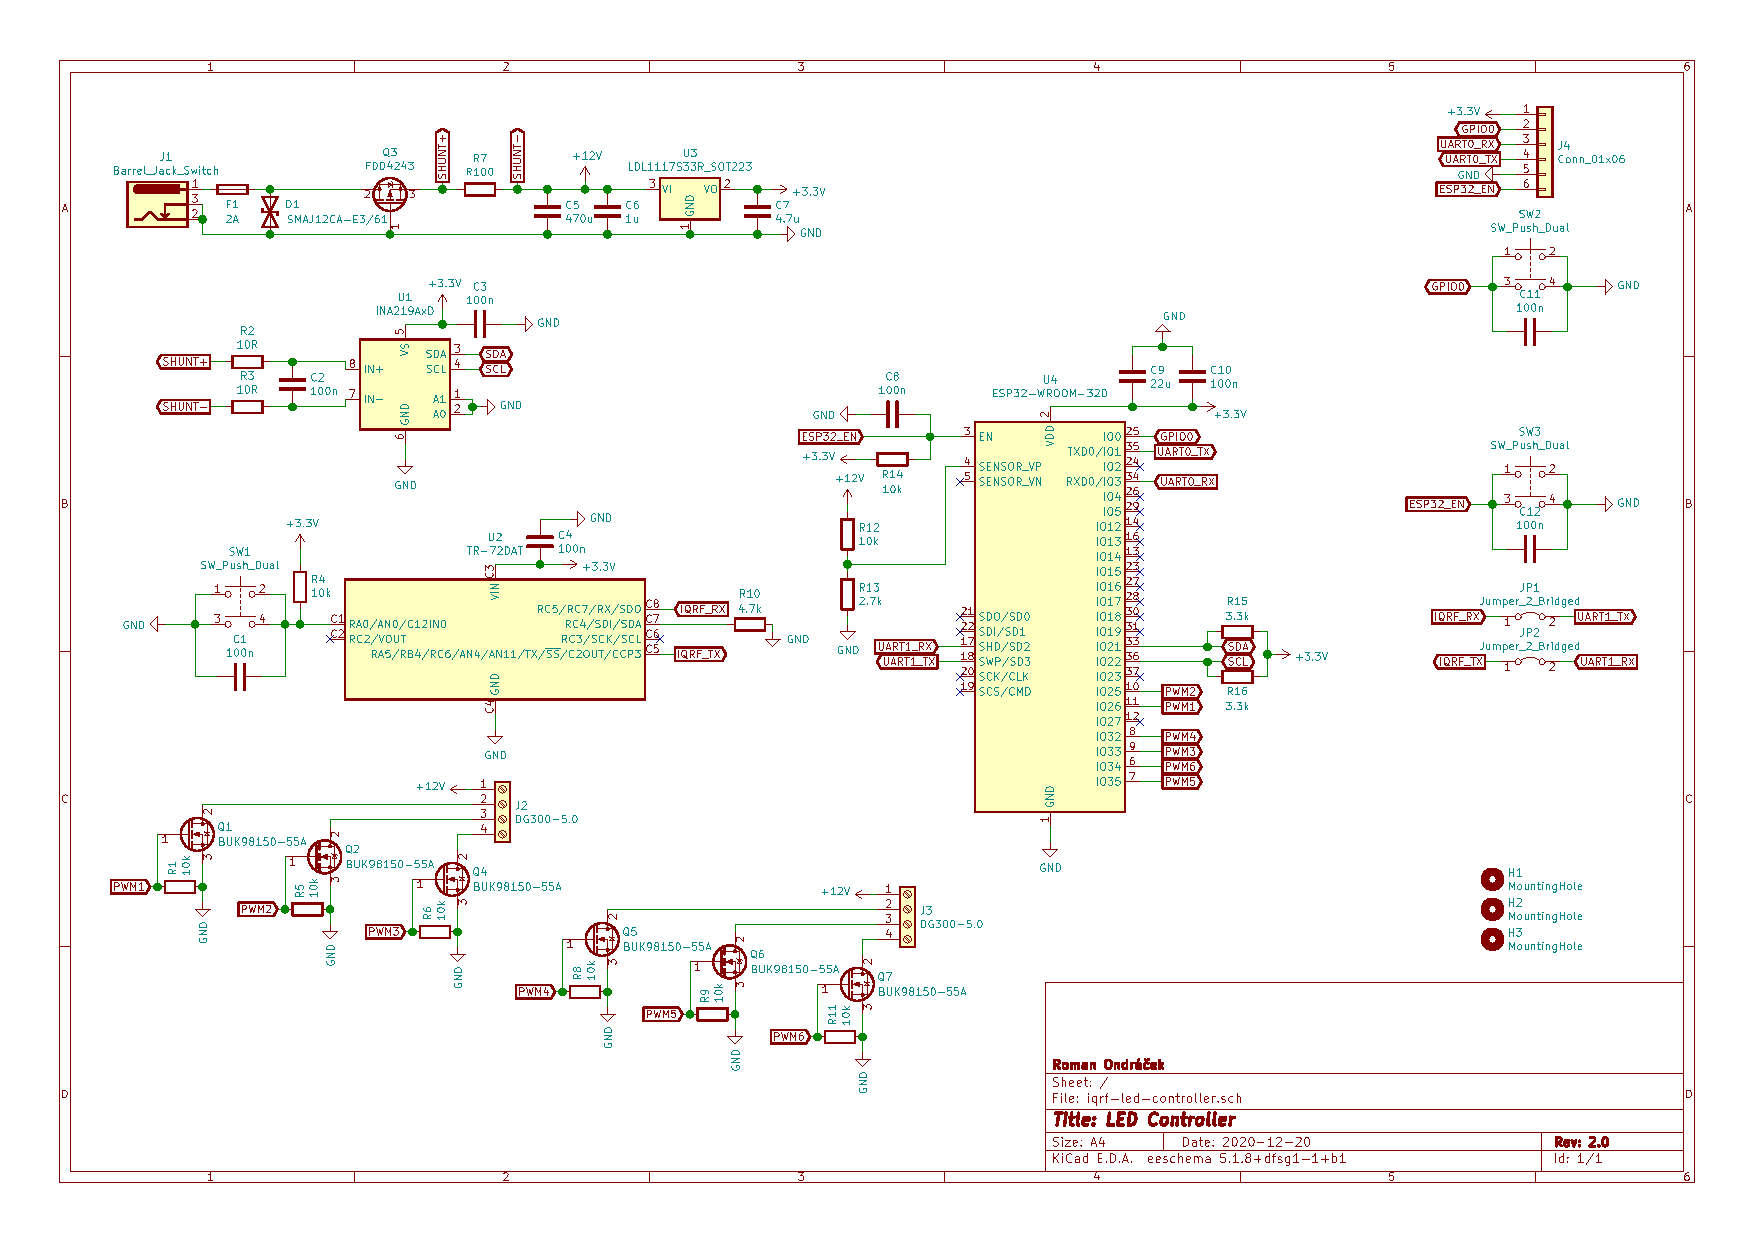
\includegraphics[scale=0.8,angle=90]{img/schema.pdf}	
	
	\newpage	
	
	\section{Způsob řešení}	
	
	O veškerou logiku se stará ESP32, které komunikuje s IQRF modulem po sběrnici UART, pomocí ADC a odporového děliče měří vstupní napětí a pomocí PWM reguluje intenzitu osvětlení. Části programu pro ESP32 byly převzaty z dokumentace aplikačního rámce ESP-IDF\footnote{\url{https://docs.espressif.com/projects/esp-idf/en/latest/esp32/index.html}}. Části Custom DPA handleru byly převzaty z ukázek z IQRF Startup balíčku\footnote{\url{https://static.iqrf.org/IQRF_Startup_Package_OS404D_TR-7xD_200918.zip}}.
	
	\section{Závěr}
	
	Navržený systém řízení a měření LED pásků byl navržen a realizován ve formě funkčního vzorku. Bohužel jsem nestihl implementovat komunikaci se senzorem proudu INA219 po sběrnici I2C, chybí profily GATT pro manipulaci s intenzitou osvětlení barevných kanálů jednotlivých LED pásků, chybí implementace IQRF standardů pro světla a ve standardu pro senzory chybí vyčítání vstupního napětí. Dále v návrhu desky plošných spojů je chyba, které znemožňuje použití 2. a 3. kanálu pro 2. RGB LED pásek.
	
	Video naleznete na \url{https://www.romanondracek.cz/imp.mp4}.
\end{document}